\chapter{Implementation in TRNSYS}

The last chapter regard the implementation in TRNSYS. At this point, remain to define the thermal model that can be done following the tutorial of TRNSYS3D plug-in for SketchUp in the TRNSYS documentation folder:
\begin{center}
....\textbackslash Trnsys17\textbackslash Documentation\textbackslash A4\_3DBuildingTutorial.pdf
\end{center} 
However, skip the preparation of the thermal model and use the TRNSYS deck (tutorial\_imported.tpf) provided within the file example. The TRNSYS deck has been created from one of the default project suggested by TRNSYS when a new project is selected. To this default deck four new elements have been added, the TypeDLT and three equations, to reach the configuration in  Figure \ref{img5:deck}. 
\begin{figure}[H]
\centering
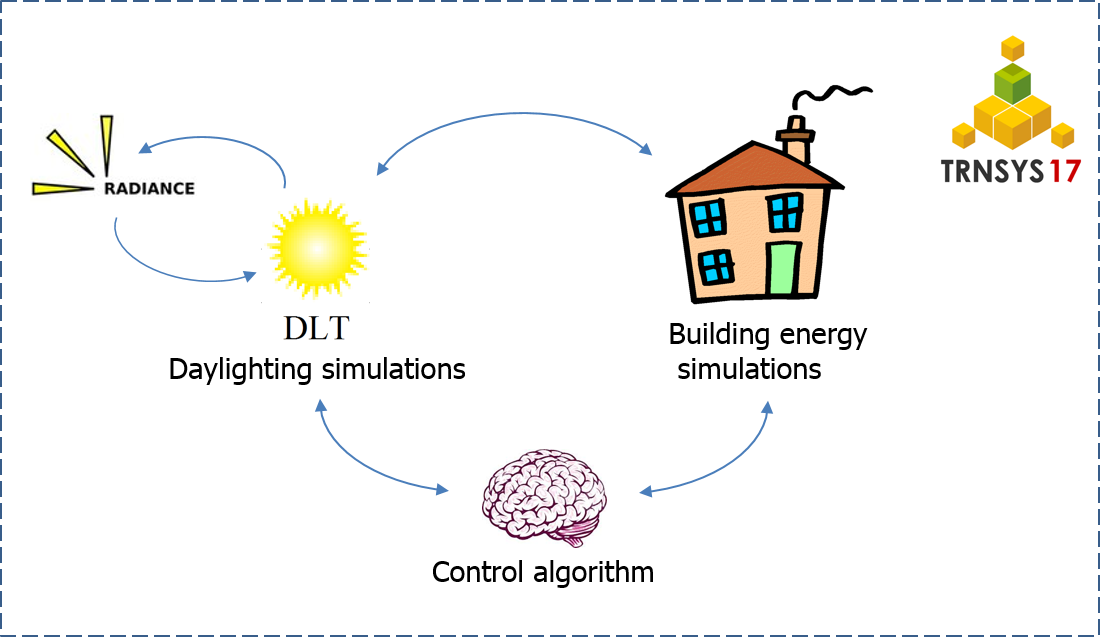
\includegraphics[width=1\textwidth]{deck}
\caption{\label{img5:deck} TRNSYS deck with the TypeDLT}
\end{figure}
One equation is used to define the control algorithm (DLT\_control), one is used to calculate the external gain due to artificial light (Light gains) of dimmed system and is direct connected to the Type56, the last equation is used to convert the shading state chose by the control in a shading factor-Fc (State2Fc) value that is passed to the Type56 and reduce of a certain percentage the transparent area of the window.\\
Copy and paste the "Zone1" folder containing the daylighting model within the project folder as specified in the Chapter \ref{sec:manualtweaks}. If you are not sure of the correct ending of the previous steps please compare your Zone1 folder with the one provided. \\
In the deck provided the input data have been already connected. Please note that from the "Weather data" Type are connected:
\begin{itemize}
\renewcommand{\labelitemi}{\tiny$\blacksquare$}
\item Latitude and Longitude 
\item Direct normal and diffuse horizontal illuminance
\item Month, day of the month and hour of the day
\end{itemize}  
Double clicking on the TypeDLT icon, observe that the Zone ID is set on 1 corresponding to name of the folder "Zone1". In addition, the Control is connected with the Equation Type "DLT\_control".\\
In Chapter \ref{sec:cfs} four files BSDF have been create. In particular, the file 0.xml correspond to the base configuration without shadings, the 1.xml, 2.xml and 3.xml correspond respectively to the configurations with shading tilted at 0, 45 and 90 degree angle.

\begin{figure}[h]
\centering
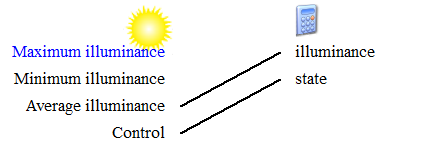
\includegraphics[width=0.6\textwidth]{controlinput}
\caption{\label{img5:controlinput} Input control equation}
\end{figure}

The control strategy of this system is based on the daylight availability within the zone and takes in input two parameters: average illuminance and control (current shading state), see Figure \ref{img5:controlinput}. The aim is to find the shading state that provide an internal illuminance within the range 300-3000 lux. The state does not change if the threshold limits are already respected.\\
The "State2Fc" equation takes in input the current shading state and gives in output a Fc value that represent the percentage of opaque area due to the shading respect to the glazing surface. Then, the Fc is passed to the Type56 as external shading factor (Figure \ref{img5:windowtrnsys}). Notice also that the glazing system created in WINDOW7.3 has been imported in TRNSYS and used in the simulation. \\
For the conversion of shading state into shading factor the energy balance in the equation \ref{eq:fc} has been used.

\begin{equation}\label{eq:fc}
Fc = 1 - \dfrac{SHGC \tb{glass+shading}}{SHGC \tb{glass}}
\end{equation}

where SHGC \tb{shading+glass} and SHGC \tb{glass} are the Solar Heat Gain Coefficients respectively of the whole systems, glazing and shading, and of the glazing system only. Both these values are calculated by WINDOW 7.3. 

\begin{figure}[h]
\centering
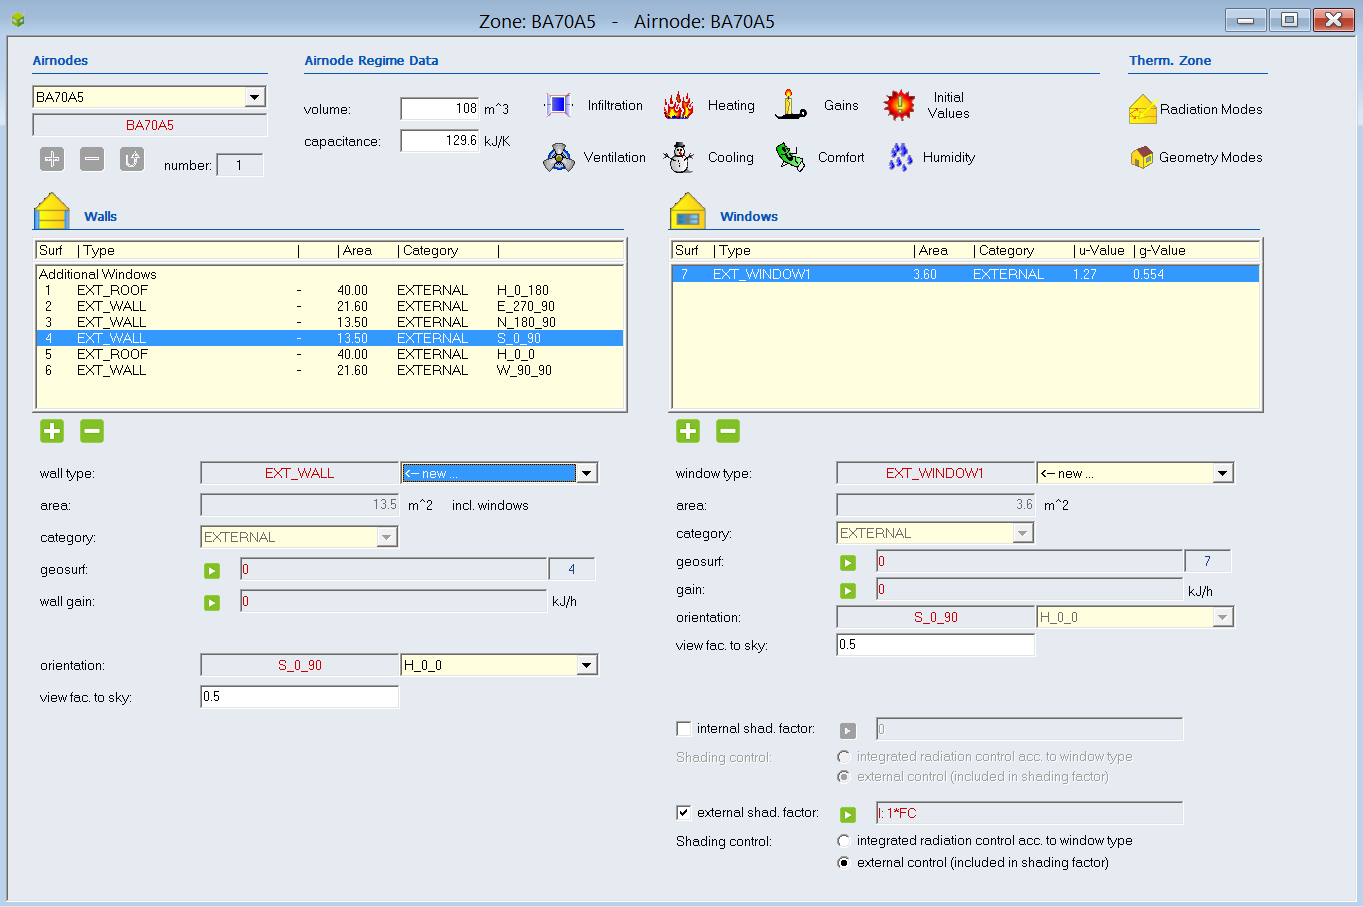
\includegraphics[width=0.7\textwidth]{windowtrnsys}
\caption{\label{img5:windowtrnsys} Zone window - Fc input as external shading factor}
\end{figure}

\begin{figure}[H]
\centering
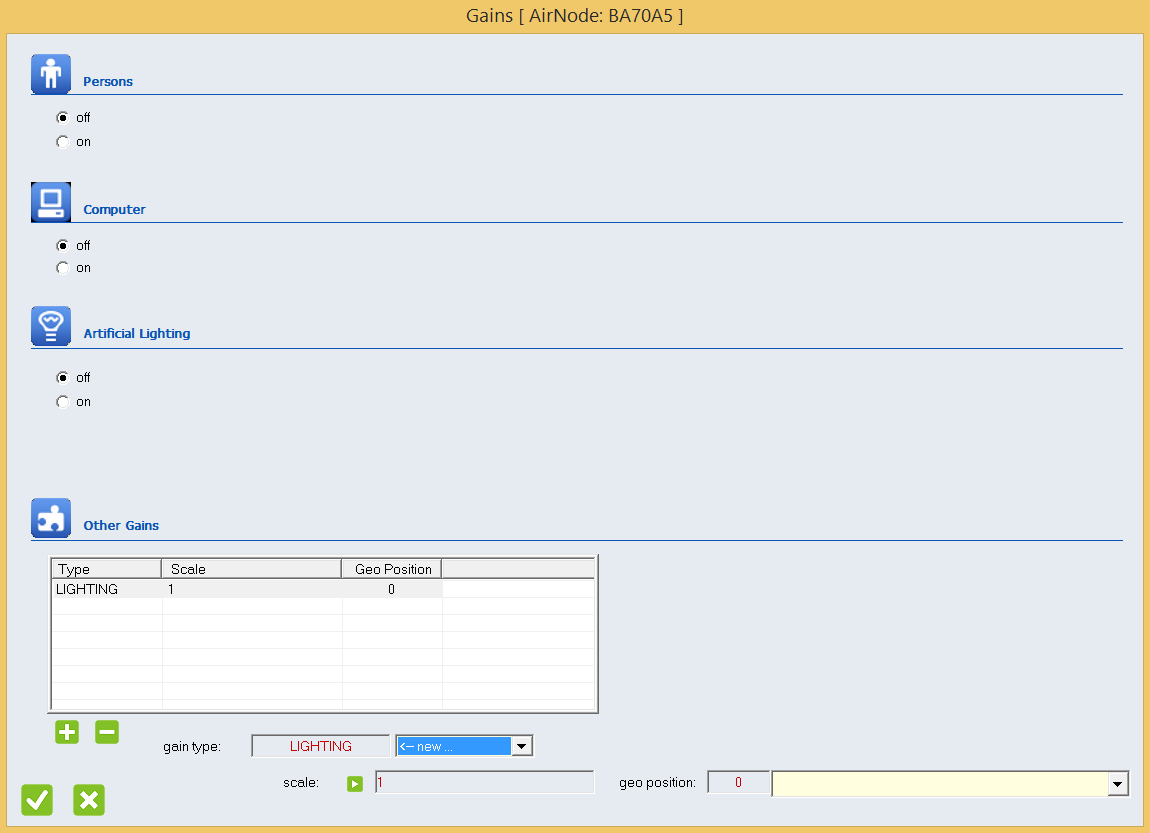
\includegraphics[width=0.7\textwidth]{gain}
\caption{\label{img5:gain} Gain window - The Artificial lighting gain is considered as Other gain from the TRNSYS deck}
\end{figure}

The gains due to the artificial lighting are calculated through an ad hoc equation. The equation "Light gains" takes in input the minimum illuminance level over the sensors grid from the TypeDLT and if the natural light is lower than the threshold value of 500 lux the artificial light is dimmed to reach this level. The artificial light power required to arrive at 500 lux is converted in heat gain and passed at each time step to the Type56 as external gain (Figure \ref{img5:gain}). \\
Once explained how the deck works let's simulate. Click \textit{Calculate -> Run simulation [F8]}, first the view and daylighting matrices will be calculate (Figure \ref{img5:matrices}). The matrices generation requires several  minutes depending also by the complexity of the geometry.

\begin{figure}[h] 
\centering
  \subfigure[View matrix generation]{% 
    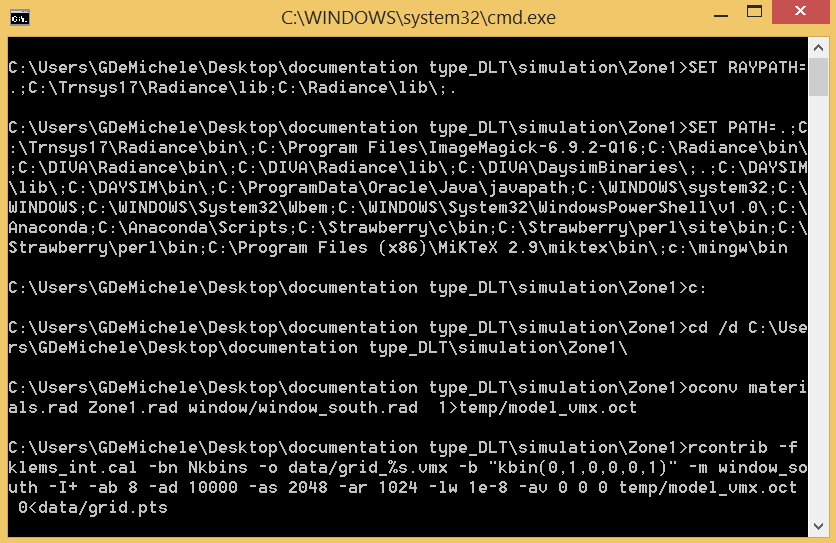
\includegraphics[width=.45\textwidth]{vmx} \label{img5:vmx} 
  } 
  \subfigure[Daylighting matrix generation]{% 
    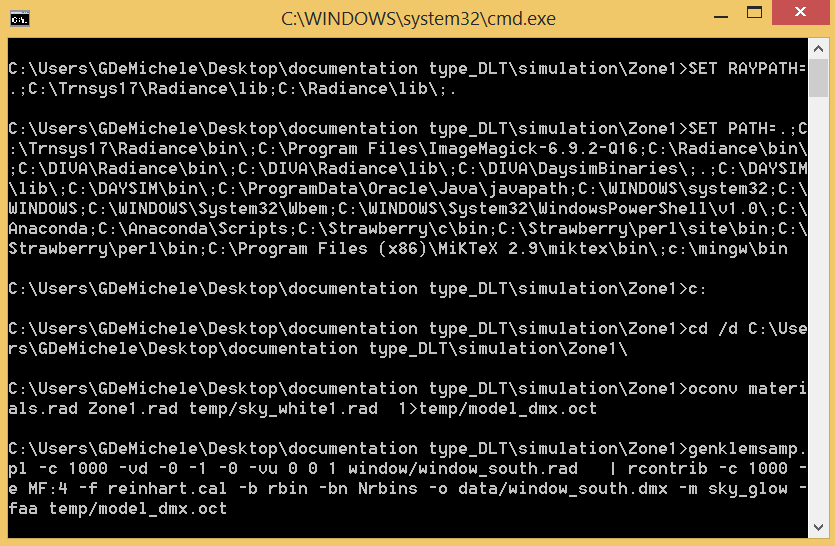
\includegraphics[width=.45\textwidth]{dmx} \label{img5:dmx} 
  }
  \caption{\label{img5:matrices} View and daylighting matrix generation}
\end{figure}

At each time-step will be created the sky vector and performed the matrices multiplication (Figure \ref{img5:3pm}) that require few seconds. Within the time step the control decides if change state and run another daylighting simulation or go ahead with the thermal simulation and the next time step.

\begin{figure}[h]
\centering
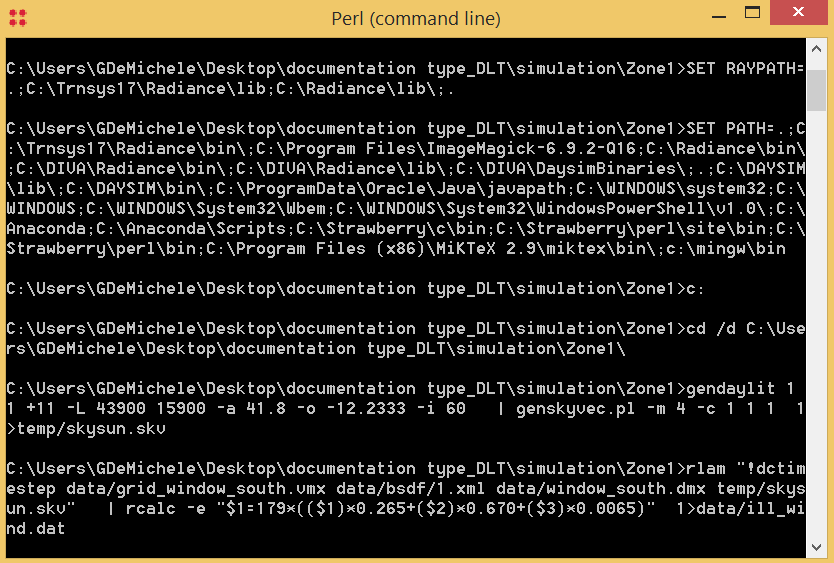
\includegraphics[width=0.5\textwidth]{3pm}
\caption{\label{img5:3pm} Sky vector generation and matrix multiplication }
\end{figure}


%Once the model is ready, create a new project in the Simulation Studio and locate the TypeDLT onto the TRNSYS deck. First, connect the following variable from the \textit{Weather data} Type: 
%\begin{itemize}
%\renewcommand{\labelitemi}{\tiny$\blacksquare$}
%\item Latitude and Longitude 
%\item Direct normal and diffuse horizontal illuminance
%\item Month, day of the month and hour of the day
%\end{itemize} 
%
%\begin{figure}[h]
%\centering
%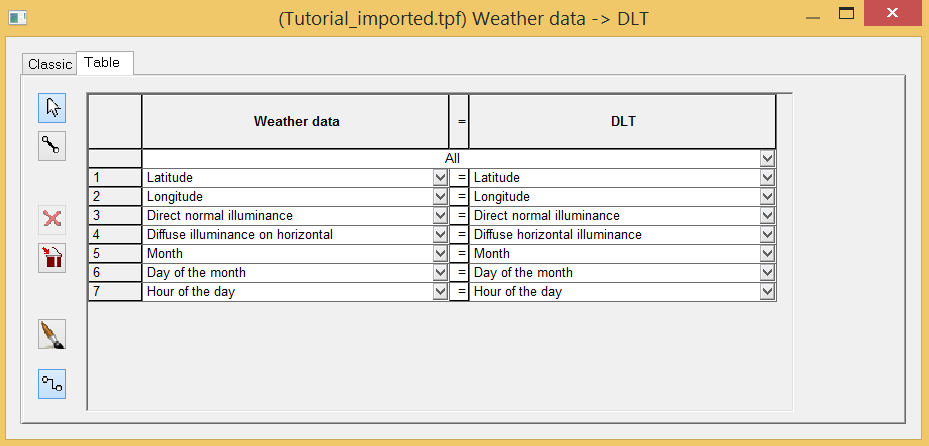
\includegraphics[width=0.7\textwidth]{DLTint}
%\caption{\label{img5:DLTint} Connections between Weather data and TypeDLT}
%\end{figure}
%
%
%Double click on the TypeDLT icon, set within the Type's control panel the Zone ID that correspond to the integer number that you have assigned in the previous section to the folder which contain the Radiance files. The default values is 1 (Figure \ref{img5:DLTinput}).
%
%\begin{figure}[h]
%\centering
%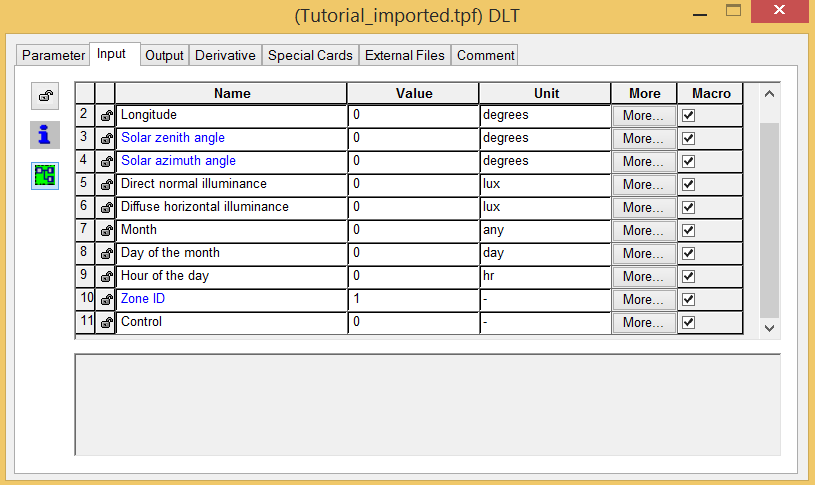
\includegraphics[width=0.7\textwidth]{DLTinput}
%\caption{\label{img5:DLTinput} Input window TypeDLT}
%\end{figure}
%
%At this point, the TypeDLT is ready to simulate and the user can connect the Type's outputs and inputs following its needs.\\
%\begin{figure}[h]
%\centering
%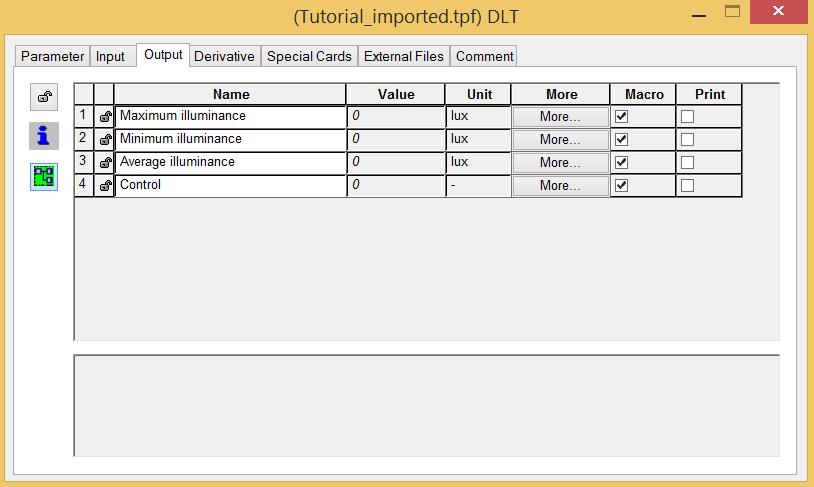
\includegraphics[width=0.7\textwidth]{DLToutput}
%\caption{\label{img5:DLToutput} Output window TypeDLT }
%\end{figure}
%Once the TRNSYS deck is ready and the first simulation is run the view and daylighting matrices (see the manual for the theory) are generated and two terminal windows will be opened, Figure \ref{img5:matrices}.
%
%\begin{figure}[h] 
%\centering
%  \subfigure[View matrix generation]{% 
%    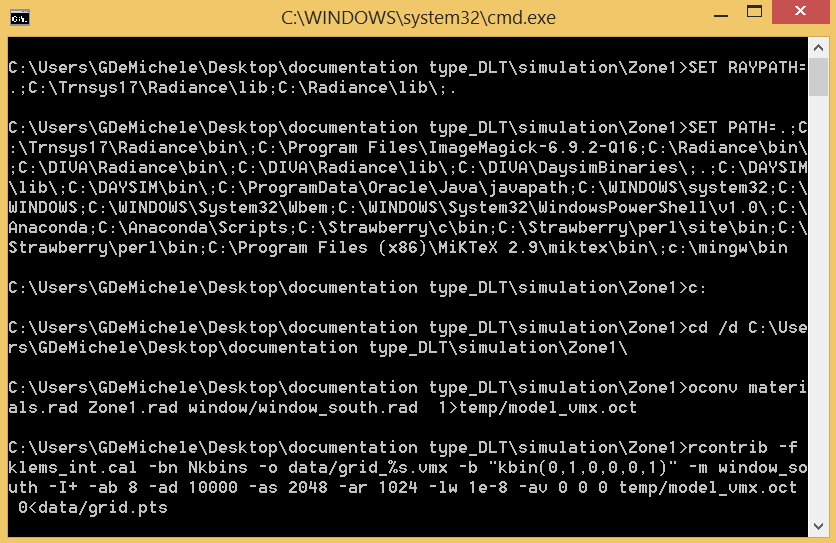
\includegraphics[width=.45\textwidth]{vmx} \label{img5:vmx} 
%  } 
%  \subfigure[Daylighting matrix generation]{% 
%    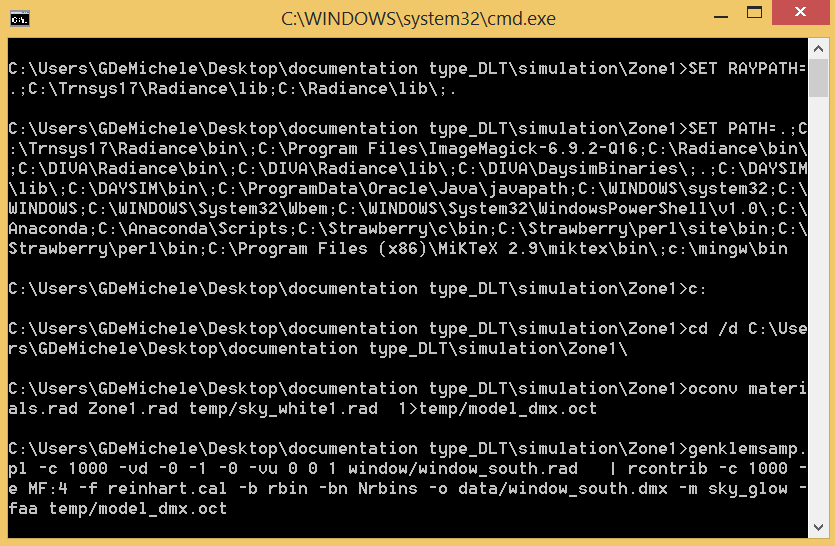
\includegraphics[width=.45\textwidth]{dmx} \label{img5:dmx} 
%  }
%  \caption{\label{img5:matrices} Terminals opened for the view and daylighting matrix generation}
%\end{figure}
%
%The matrices generation requires several  minutes depending also by the complexity of the geometry. Once the matrices are crated it is not necessary to regenerate them for each time-step and for next simulations of the same Radiance scene. At each time-step will be created the sky vector and performed the matrices multiplication (Figure \ref{img5:3pm}) that require few seconds.
%
%\begin{figure}[h]
%\centering
%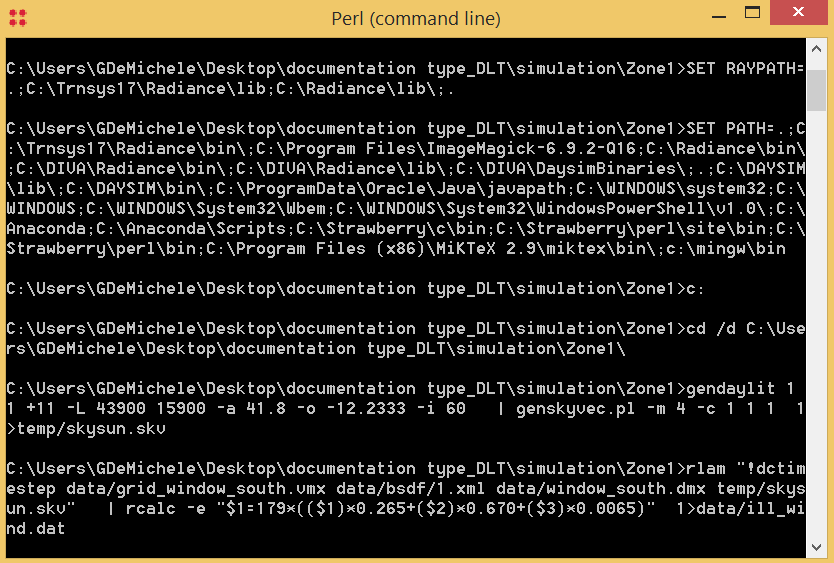
\includegraphics[width=0.5\textwidth]{3pm}
%\caption{\label{img5:3pm} Terminal window - Sky vector generation and matrix multiplication }
%\end{figure}
%
%It is very important to know that the *.vmx and *.dmx file generated are not overwrite in any case, therefore if you need to regenerate these files delete them manually in the folder \textit{data}.\\
%In the following section the example file provided is used to show some of the functionalities offered by the TypeDLT.



%\section{File Example}
%In the example will be shown how to use the outputs for the control of a dynamic shading system and for the calculation of the heat gain due to artificial light. The TRNSYS deck has been created from one of the default project suggested by TRNSYS when a new project is selected. To this default deck four new elements have been added, the TypeDLT and three equations, to reach the configuration in  Figure \ref{img5:deck}. One equation is used to define the control algorithm (\textit{DLT\_control}), one is used to calculate the external gain due to artificial light (\textit{Light gains}) of dimmed system and is direct connected to the Type56, the last equation is used to convert the shading state chose by the control in a shading factor-Fc (\textit{State2Fc}) value that is passed to the Type56 and reduce of a certain percentage the transparent area of the window.
%
%\begin{figure}[H]
%\centering
%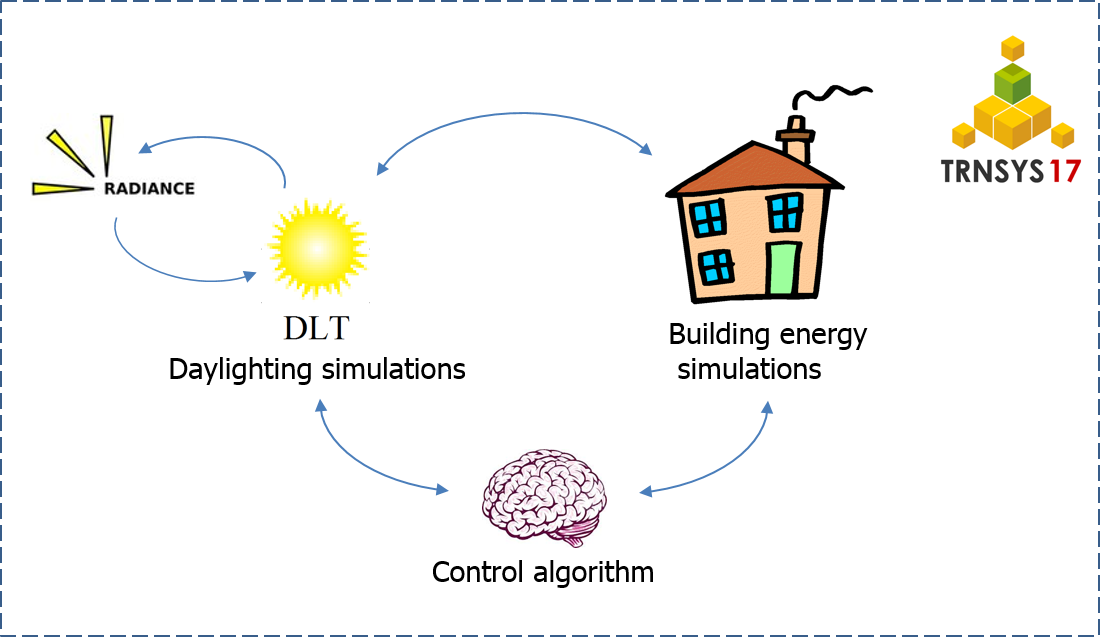
\includegraphics[width=1\textwidth]{deck}
%\caption{\label{img5:deck} TRNSYS deck with the TypeDLT}
%\end{figure}
%
%A dynamic shading systems with external flat lamellas has been considered. Four file BSDF are supplied, the file 0.xml correspond to the configuration without shadings. The 1.xml, 2.xml and 3.xml correspond respectively to the configurations with shading tilted at 0, 45 and 90 degree angle.
%
%
%\begin{figure}[h]
%\centering
%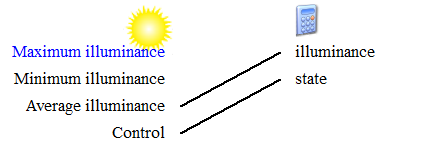
\includegraphics[width=0.6\textwidth]{controlinput}
%\caption{\label{img5:controlinput} Input control equation}
%\end{figure}
%
%The control strategy of this system is based on the daylight availability within the zone and takes in input two parameters: average illuminance and control (current shading state), see Figure \ref{img5:controlinput}. The aim is to find the shading state that provide an internal illuminance within the range 300-3000 lux. The state does not change if the threshold limits are already respected.
%
%The \textit{State2Fc} equation takes in input the current shading state and gives in output a Fc value that represent the percentage of opaque area due to the shading respect to the glazing surface. Then, the Fc is passed to the Type56 as external shading factor (Figure \ref{img5:windowtrnsys}). Notice also that the glazing system created in WINDOW7.3 has been imported in TRNSYS and used in the simulation. \\
%For the conversion of shading state into shading factor the energy balance in the equation \ref{eq:fc} has been used.
%
%\begin{equation}\label{eq:fc}
%Fc = 1 - \dfrac{SHGC \tb{glass+shading}}{SHGC \tb{glass}}
%\end{equation}
%
%where SHGC \tb{shading+glass} and SHGC \tb{glass} are the Solar Heat Gain Coefficients respectively of the whole systems, glazing and shading, and of the glazing system only. Both these values are calculated by WINDOW 7.3. 
%
%\begin{figure}[h]
%\centering
%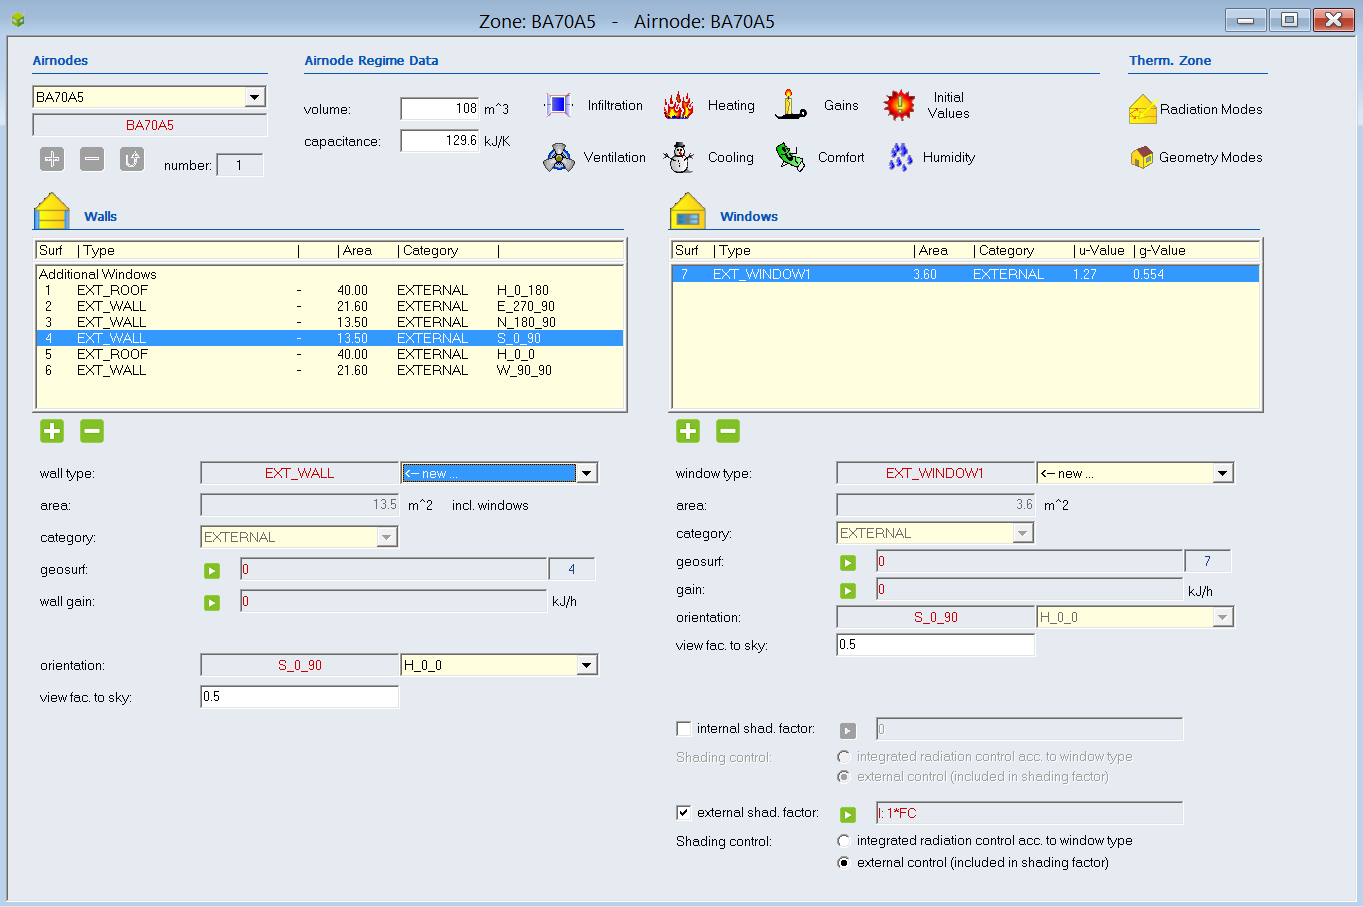
\includegraphics[width=0.7\textwidth]{windowtrnsys}
%\caption{\label{img5:windowtrnsys} Zone window - Fc input as external shading factor}
%\end{figure}
%
%\begin{figure}[h]
%\centering
%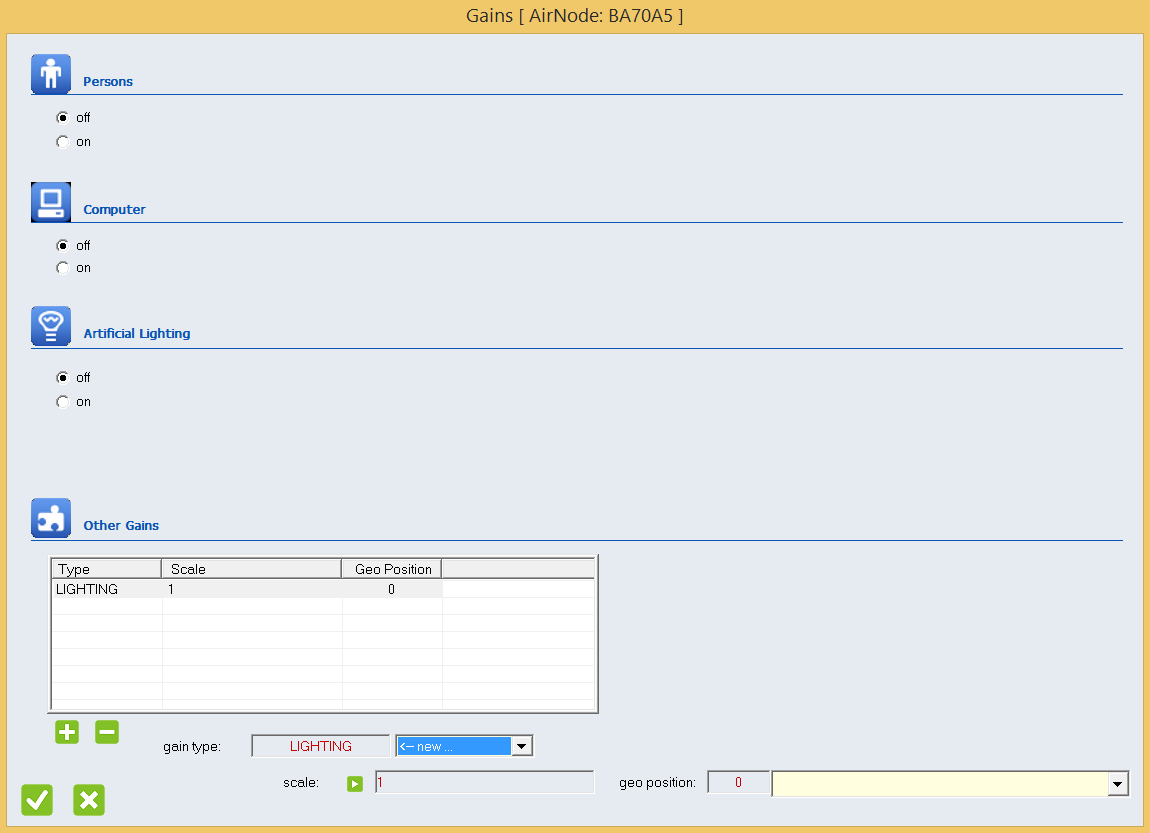
\includegraphics[width=0.7\textwidth]{gain}
%\caption{\label{img5:gain} Gain window - The Artificial lighting gain is considered as Other gain from the TRNSYS deck}
%\end{figure}
%
%The gains due to the artificial lighting are calculated through an ad hoc equation. The equation takes in input the minimum illuminance level over the sensors grid from the TypeDLT and if the natural light is lower than the threshold value of 500 lux the artificial light is dimmed to reach this level. The artificial light power required to arrive at 500 lux is converted in heat gain and passed at each time-step to the Type56 as external gain (Figure \ref{img5:gain}). 


